\section{Репликация ДНК: репликация линейных и кольцевых молекул ДНК, 
Затравка для ДНК-полимеразы, праймирование, фрагменты Оказаки. 
Ферменты, необходимые для репликации ДНК (полимеразы I и III, топоизомеразы, хеликаза, лигаза, 
праймаза, ssb). 
Теломеры и центромеры эукариот. Ориджины репликации бактерий. Белки определяющие начало 
репликации бактерий (DnaABC, ssb, SeqA, dam) Репликация кольцевых молекул ДНК по Тета –типу и по типу катящегося колеса}


\textbf{Репликация ДНК} - процесс создания двух дочерних молекул ДНК на основе одной родительской молекулы ДНК. 

Двухцепочечная молекула ДНК может быть линейной (у эукариот, организмов, клетки которых имеют  клеточное ядро) или свернутой в кольцо (у прокариот, клетки которых не имеют ядра). 

Про особенности репликации двухцепочечных линейных и кольцевых молекул см. ниже.

\subsection{Общее описание механизма репликации}
Репликация начинается в месте (сайте) инициации репликации с расплетания двойной спирали ДНК, при этом формируется репликационная вилка (см. рис. \ref{fig:3_replication_main}). В репликационной вилке ДНК копирует крупный белковый комплекс (реплисома), ключевым ферментом которого является ДНК-полимераза (см. следующий раздел).

ДНК-полимераза может присоединять свободно плавающие нуклеотиды в цепь ДНК на основе уже имеющейся цепи ДНК. Но ДНК-полимераза не умеет поставить первый нуклеотид, поэтому ей нужна \textbf{затравка} в виде короткого фрагмента РНК - \textbf{праймера} - уже сидящего на шаблонной ДНК. К его 5' концу ДНК-полимераза уже присоединяет первый дезоксирибонуклеотид и начинает полимеризовать цепь.

ДНК-полимераза умеет присоединять только 5' конец предыдущего дезоксирибонуклеотида к 3' концу следующего дезоксирибонуклеотида, поэтому относительно исходной цепи ДНК репликация доджна происходить в направлении от 3' конца к 5' концу. Тогда из двух цепей расплетающейся материнской ДНК только одна направлена так, что ДНК-полимераза может непрерывно синтезировать новую цепь. Получающаяся непрерывно дочерняя цепь  называется \textbf{лидирующей}. Вторая же цепь называется \textbf{отстающей}. 

Отстающая цепь синтезируется так. На метеринскую цепь ДНК праймазой (специальным белком) ставится праймер, на него садится ДНК-полимераза, синтезирует небольшой участок ДНК - \textbf{фрагмент Оказаки} - в обратном направлении относительно расплетания материнской ДНК и отваливается. Затем такие фрагменты соединяет лигаза (тоже специальный фермент), а праймер заменяется на участок ДНК. За это время репликационная вилка уехала вперед, и праймаза ставит новый праймер поближе к вилке, процесс повторяется.

В каждом сайте может формироваться одна или две репликационные вилки в зависимости от того, является ли репликация одно- или двунаправленной. Более распространена двунаправленная репликация. Через некоторое время после начала репликации в электронный микроскоп можно наблюдать репликационный глазок — участок хромосомы, где ДНК уже реплицирована, окружённый более протяжёнными участками нереплицированной ДНК.

 Репликационная вилка движется со скоростью порядка 100 000 пар нуклеотидов в минуту у прокариот и 500—5000 — у эукариот.

\begin{figure}[h!]
    \centering
    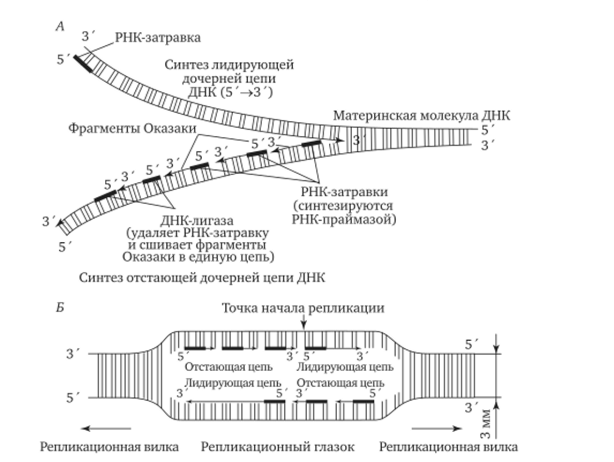
\includegraphics[width = 0.8 \linewidth]{3_replication_main.png}
    \caption{Схема репликационной вилки (выше) и репликационного глазка (ниже). Репликационная вилка на втором рисунке - область, где материнская двухцепочечная молекула расходится на две. Стрелочками обозначено то, что вилки удаляются друг от друга, двигаясь по материнской (шаблонной) ДНК в направлении от 3' к 5' концам.}
    \label{fig:3_replication_main}
\end{figure}

\subsection{Ферменты, необходимые для репликации ДНК}

\begin{itemize}

    \item \textbf{Топоизомераза} - фермент, раскручивающий спираль ДНК. Едет вдоль закрученной двойной спирали ДНК и ставляет за собой две водородно связанные цепочки ДНК, лежащие в одной плоскости. (здесь и далее смотреть на картинку \ref{fig:3_rep}).
    
    \item \textbf{Хеликаза} - фермент, рвущий водородные связи между двумя цепочками ДНК. Едет за топоизомеразой по двум связанным цепям ДНК и оставляет за собой две несвязанные цепи ДНК.
    
    \item \textbf{Полимераза} (ДНК полимераза) - фермент, полимеризующий молекулу ДНК. Всегда едет по цепи ДНК в направлении 3'-5', смотрит на нее как на шаблон и достраивает комплиментарную ей цепь из свободно плавающих дезоксирибонулеотидов. 
    
    ДНК-полимераз существует несколько типов. У бактерий \textbf{ДНК-полимераза I} удаляет РНК-фрагменты на отстающей цепи и ставит на их место ДНК, \textbf{ДНК-полимераза II} участвует в репарации (восстановлении сломанных кусочков) ДНК, \textbf{ДНК-полимераза III} просто основной фермент (именно она делает почти всю работу в синтезировании ДНК с лидирующей и отстающей цепей).
    
    \item \textbf{Лигаза} (ДНК-лигаза) - фермент, ковалентно сшивающий цепи ДНК в местах разрыва. Едет по отстающей цепи ДНК и сшивает фрагменты ОКазаки. 
    
    \item \textbf{Праймаза} - фермент, синтезирующий РНК-затравку (праймер) — короткий фрагмент РНК, которая является инициатором в работе ДНК-полимеразы (полимераза не способна синтезировать ДНК с нуля, но может добавлять нуклеотиды к уже имеющимся). 
    
    \item \textbf{SSB-белки} - ферменты, предотвращающие диссоциацию полимеразы от матрицы ДНК и повышающие эффективность ее работы. Окружают кольцом ДНК и «скользят» по ней вместе с продвигающимся вперед ферментом ДНК-полимеразы. 
    
    \begin{figure}[h!]
        \centering
        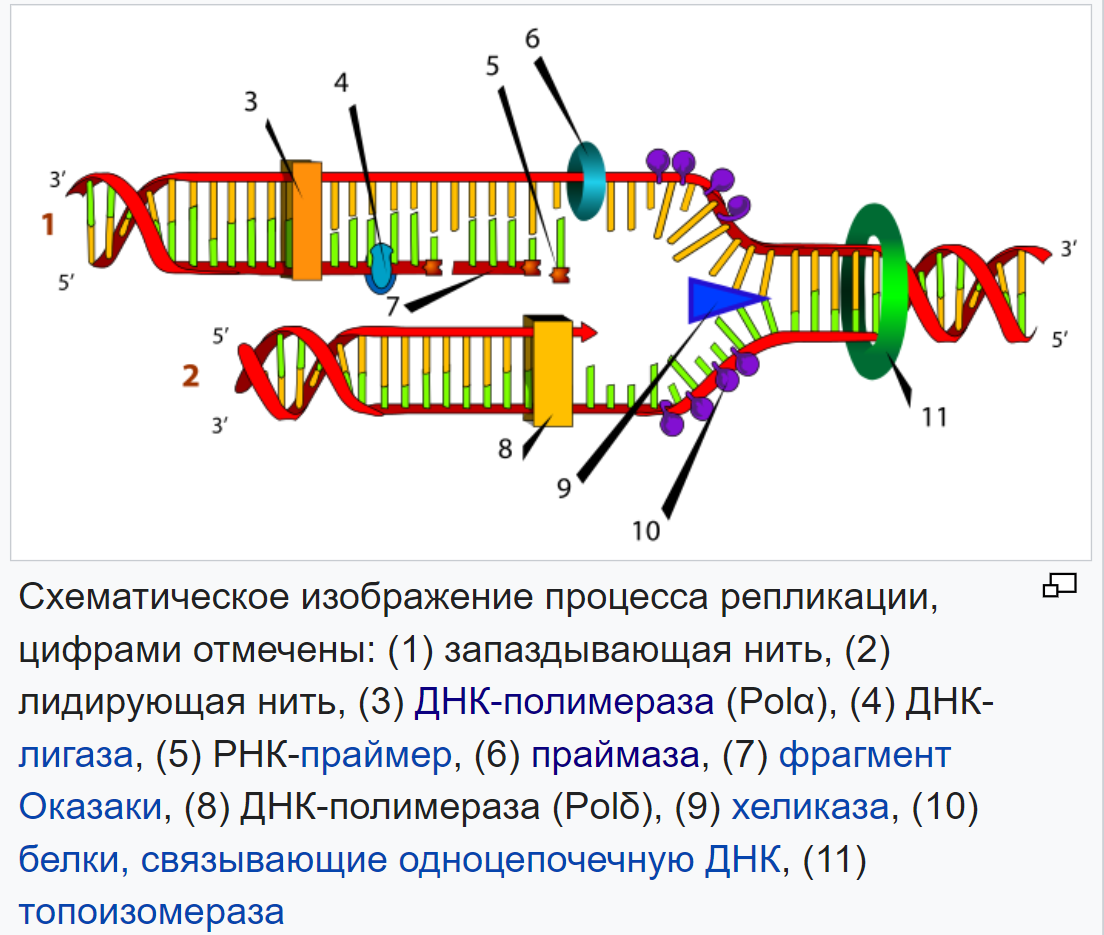
\includegraphics[width=0.7\linewidth]{3_replication.png}
        \caption{Белки, участвующие в процессе репликации}
        \label{fig:3_rep}
    \end{figure}
    
\end{itemize}

\subsection{Теломеры и центромеры эукариот}
\textbf{Теломеры} - концевые участки хромосом. Теломерные участки хромосом характеризуются отсутствием способности к соединению с другими хромосомами или их фрагментами и выполняют защитную функцию. 

В каждом цикле деления теломеры клетки укорачиваются из-за неспособности ДНК-полимеразы синтезировать копию ДНК с самого конца. Она в состоянии лишь добавлять нуклеотиды к уже существующей 3’-гидроксильной группе. Данный феномен носит название концевой недорепликации и является одной из важнейших причин биологического старения.

Тем не менее, вследствие этого явления теломеры должны укорачиваться весьма медленно — по несколько (3-6) нуклеотидов за клеточный цикл.

\begin{figure}[h!]
    \centering
    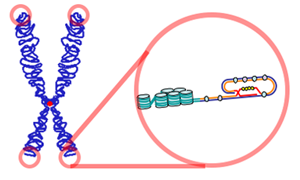
\includegraphics[]{3_telomere.png}
    \caption{Концевые участки хромосом, теломеры}
    \label{fig:3_telomere}
\end{figure}

\textbf{Центромеры} - участок хромосомы, который связывает сестринские хроматиды, играет важную роль в процессе деления клеточного ядра и участвует в контроле экспрессии генов. Характеризуется специфическими последовательностью нуклеотидов и структурой.

\begin{figure}[h!]
    \centering
    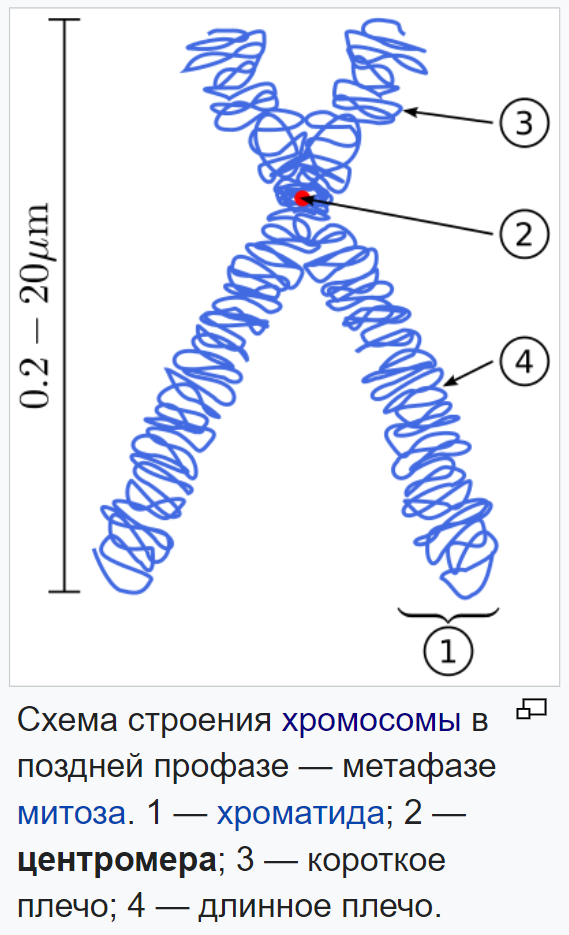
\includegraphics[width = 0.3 \linewidth]{3_centromere.png}
    \caption{Центральные участки хромосом, центромеры}
    \label{fig:3_centromere}
\end{figure}

\subsection{Ориджины репликации у бактерий}
\textbf{Точка начала репликации} (англ. origin of replication) — это фрагмент молекулы нуклеиновой кислоты, с которого начинается её репликация. Точка начала репликации и прилегающие к ней фрагменты нуклеиновой кислоты, не отделённые сайтами терминации, составляют единицу репликации — репликон. Репликация ДНК может начинаться от точки начала репликации в одном или двух направлениях.

Хромосомы и плазмиды (внехромосомный самовоспроизводящийся генетический элемент, специфичен для прокариот) прокариот (в частности, бактерий) содержат одну, реже несколько точек начала репликации ДНК (хромосомы эукариот имеют множество таких точек).

\subsection{Белки, определяющие начало репликации у бактерий}

Проиллюстрируем на примере Escherichia coli.

Генетический локус, содержащий единственную точку начала репликации хромосомы Escherichia coli (кишечной палочки), получил название oriC. OriC состоит из 245 пар оснований и включает две функциональных области: область специфичного связывания фактора инициации репликации DnaA (англ.) и область первичного раскручивания спирали ДНК — DUE (англ. DNA unwinding element). 

\subsection{Репликация кольцевых молекул ДНК по тета-типу}
Репликация по тета-механизму включает в себя следующие этапы:
\begin{itemize}
    \item 
    расплетание двух родительских цепей;
    \item
    синтез праймерной РНК (пРНК) на каждой из них;
    \item
    инициация репликации при помощи ковалентного нарастания пРНК на каждой из них;
    \item
    синтез комплементарной цепи ДНК на каждой из родительских цепей. Одна из цепей при этом выступает лидирующей, другая — отстающей, хотя синтез цепей происходит одновременно.
\end{itemize}

Тета-репликация может начинаться одновременно с одной или нескольких точек и быть при этом одно- или двунаправленной. В электронный микроскоп репликационная структура выглядит как греческая буква \(\theta\), отчего и называется тета-структурой (см. рис. \ref{fig:3_theta}).

\begin{figure}[h!]
    \centering
    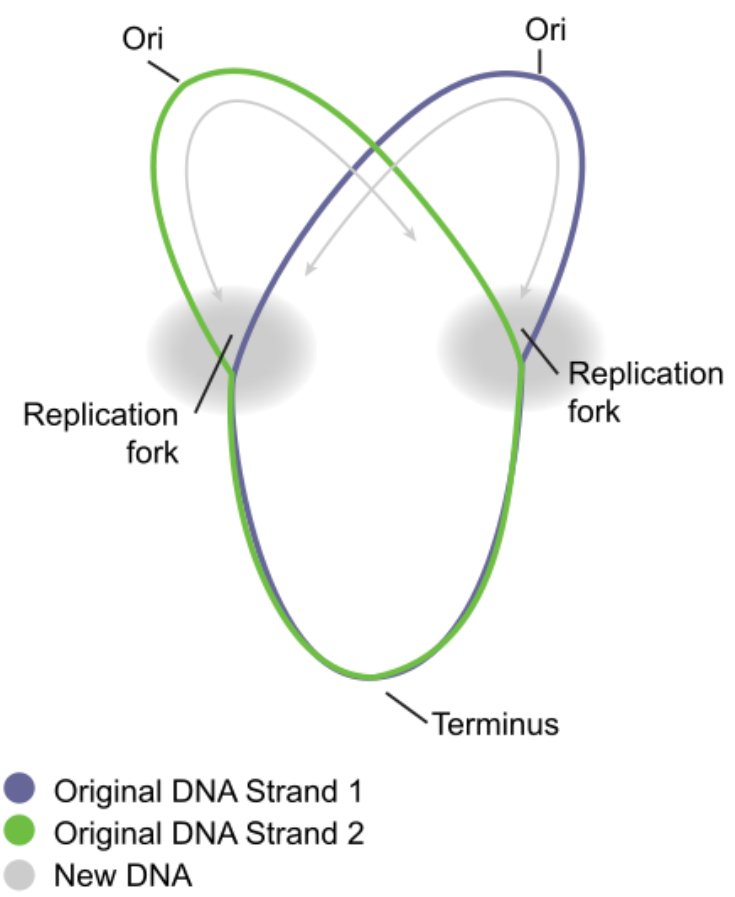
\includegraphics[width = 0.4 \linewidth]{3_theta.png}
    \caption{Этап репликации по тета-типу. Видно две репликационные вилки, разъезжающиеся друг от друга (показано стрелочками). Ori - место начала репликации (ориджин).}
    \label{fig:3_theta}
\end{figure}

\subsection{Репликация кольцевых молекул ДНК по типу катящегося колеса}
Сущность этого механизма заключается в следующем. Вначале инициаторный белок Rep совершает одноцепочечный разрыв в цепи ДНК. Появившаяся при этом свободная 3'-OH-группа служит праймером для синтеза ДНК ДНК-полимеразой III клетки-хозяина. Cинтезируется лидирующая цепь и восстанавливается двухцепочечная структура исходной ДНК. Содержащая разрыв цепь ДНК при этом удаляется, и происходит её репликация ДНК-полимеразой III, сопровождающаяся созданием праймера РНК-полимеразой. После полной репликации ДНК-полимераза I заменяет праймер на ДНК, а ДНК-лигаза сшивает концы, образуя тем самым окончательную двухцепочечную ДНК (см. \ref{fig:3_wheel}).

\begin{figure}[h!]
    \centering
    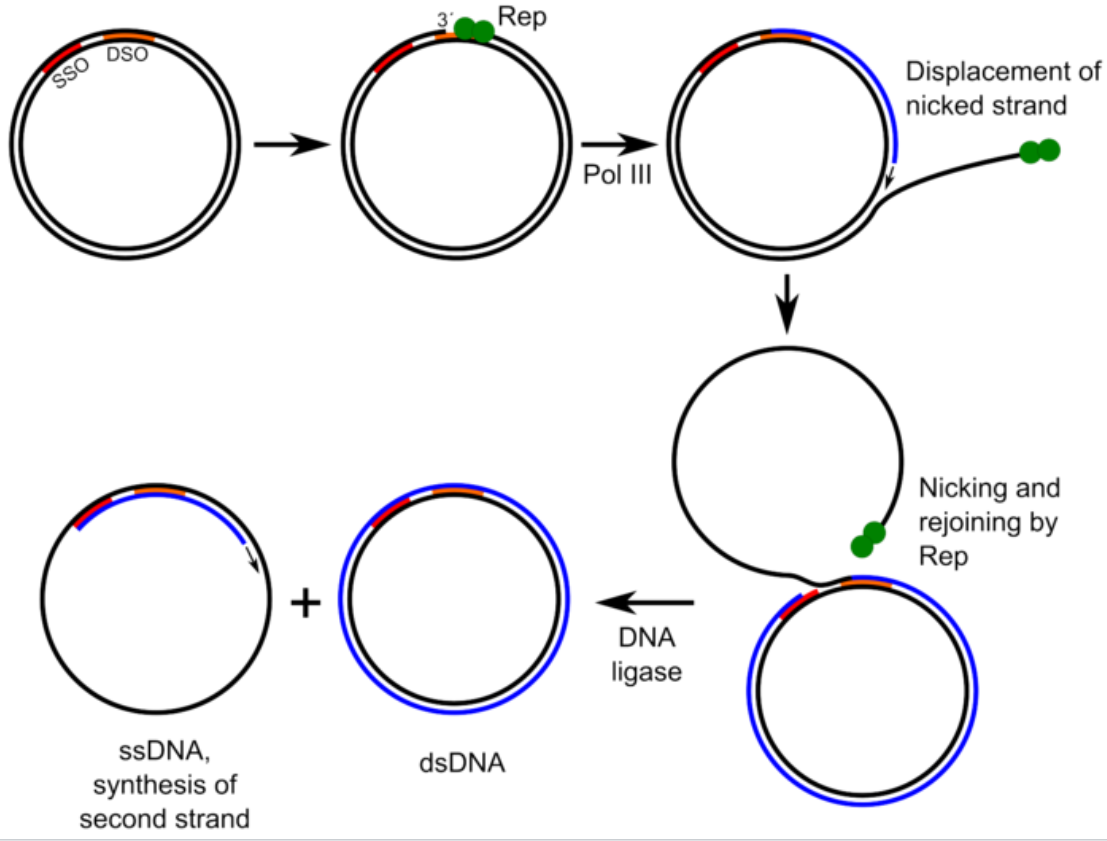
\includegraphics[width = 0.6 \linewidth]{3_wheel.png}
    \caption{Этапы репликации по типу катящегося колеса}
    \label{fig:3_wheel}
\end{figure}
